% vim: filetype=tex spell

\chapter{Verification}

\label{ch:Verification}

The \ac{ACDS} consists of experimental hardware controlled by experimental software and as such requires a significant amount of verification to make sure everything functions on orbit. Ideally everything would be verified before launch but, it is difficult to replicate the on-orbit environment closely. The magnetic field can be effectively simulated using the Helmholtz cage so the sensors can be calibrated and tested. 

\section{Motivation}

The \acp{LPMT} used for the \ac{ACDS} pose a unique challenge when compared to both passive magnetic torquers and active proportional torquers, the \acp{LPMT} switch but can't be switched off. Magnetometer measurements are used for attitude determination but the field from the torquers, if not compensated for, will overwhelm the Earth's magnetic field making attitude determination impossible.

\subsection{Torquer offsets}


\afterpage{\begin{landscape}
\begin{figure}[p]
    \centering
    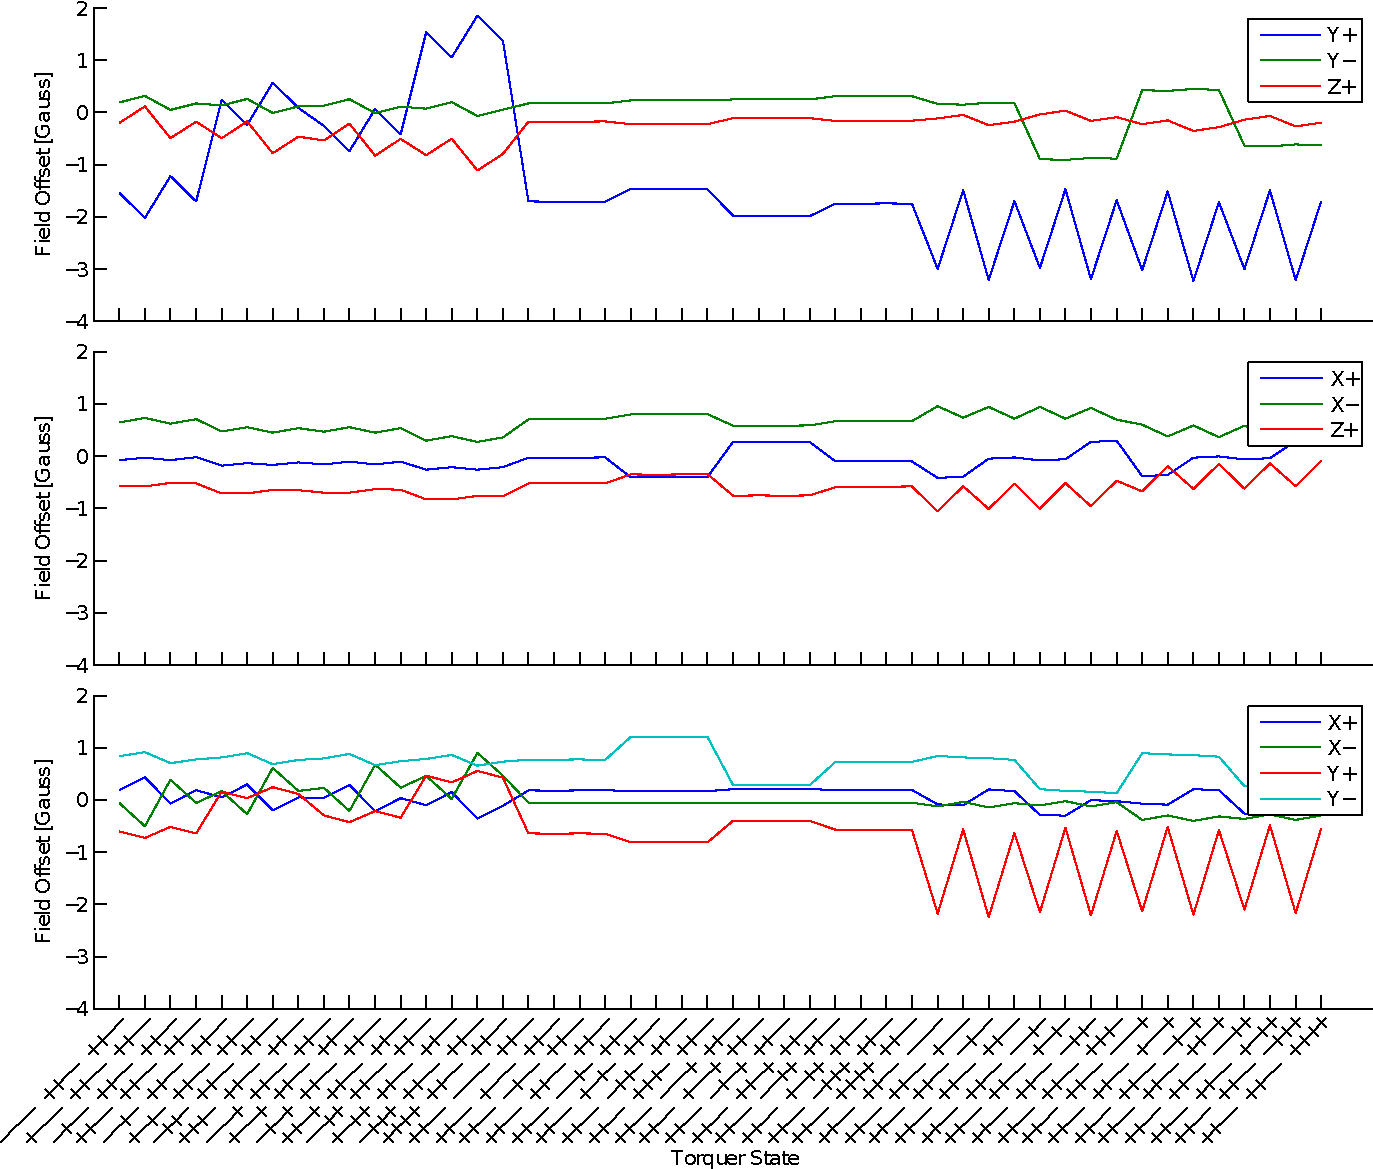
\includegraphics[width=\linewidth]{board-offsets}
    \caption{Magnetic field offsets due to changing torquer states as measured by different \acp{SPB}}
    \label{fig:b-offset}
\end{figure}
\end{landscape}}



The magnetic field of the Earth ranges from 0.3 to 0.6 Gauss \cite[pp.~114]{Wertz}. In order to measure the attitude of the \ac{ARC} to within {\textpm5\textdegree} the Earth's magnetic field must be measured with an error of less than 26~mGauss. This means that the offsets from the torquers must be known with an accuracy of at least 26~mGauss.

Because of the nature of the dipole magnetic field, the offsets measured by each magnetometer are unique to each magnetometer and torquer combination. Some torquers have only a small effect on each magnetometer and some have a much larger effect. 

To visualize the torquer offsets the torquer compensation data, explained in \cref{sec:tq-comp}, is used. The \lstinline[style=code,language=Matlab]$offsetplot$ function is used to plot the changes in torquer offset. The offset part of the compensation data is plotted with respect to torquer state.

\Cref{fig:b-offset} shows the plot from \lstinline[style=code,language=Matlab]$offsetplot$. The plot only shows the 48 torquer states used for calibration out of the 4096 possible states. The state of each torquer is indicated with a ``\texttt{+}'' if the torquer was flipped in the positive direction and a ``\texttt{-}'' if the torquer was flipped in the negative direction. The torquers are separated into groups of four torquers by axis. For the locations of torquers on the \ac{ACDS} board refer back to \cref{fig:boardRender}. The first group is for the X-axis and the last is for the Z-axis. In the first 16 states the X-axis torquers are flipped in all possible states, for the next 16 the Y-axis torquers are flipped through all possible states and for the last 16 states the Z-axis torquers are flipped through all possible states.

 
\begin{table}[!ht]
    \centering
    \caption{Information from \lstinline[style=code,language=Matlab]$offsetplot$}
    \label{tab:off-stat}
    \begin{tabular}{|c|c|c|c|}
        \hline
        \acs{SPB}&Max Offset&Min Offset&Deviation\\
        &(mGauss)&(mGauss)&(mGauss)\\
        \hline
        \multicolumn{4}{|c|}{\bfseries X-axis}\\
        \hline
        Y-&236.6&-1123.26&1359.86\\
        \hline
        Y+&2106.79&-3142.88&5249.66\\
        \hline
        Z+&874.67&-352.60&1227.26\\
        \hline
        \multicolumn{4}{|c|}{\bfseries Y-axis}\\
        \hline
        Z+&2448.90&1450.44&998.46\\
        \hline
        \multicolumn{4}{|c|}{\bfseries Z-axis}\\
        \hline
        Y-&1248.44&143.34&1105.10\\
        \hline
        Y+&606.78&-2364.76&2971.54\\
        \hline
    \end{tabular}
\end{table}

\Cref{tab:off-stat} shows the offset max and min's. The deviation is the diffrence between the max and min and is an indication of how much of an affect the torquers have on the magnetometers. The greatest deviation is just over 5~Gauss for the Y+ \ac{SPB} measuring the X-axis. The Y+ \ac{SPB} also has the second highest deviation of almost 3~Gauss. The Y- and Z+ \acp{SPB} have deviations that are closer to 1~Gauss. Looking back at \cref{fig:torquers} it makes sense that the Y+ \ac{SPB} has the largest torquer offset as it is located close to a pair of X torquers and a pair of Z-torquers. The Y- \ac{SPB} is located next to the header so the torquers are located a bit farther away. The Z+ board is located farthest away from the torquers so one would expect that the offsets for it might be significantly smaller.


\Cref{fig:b-offset,tab:off-stat} show the necessity of torquer compensation. There are large variations in the measured magnetic field due to the torquers changing state, the largest is over 5~Gauss. Without torquer compensation attitude determination would be impossible. What \cref{fig:b-offset,tab:off-stat} do not show is how repeatable the offsets are which determines if compensation is possible.

\subsection{Torquer Repeatability}

The torquer compensation method depends on the torquer offsets being repeatable. If the offsets are not very repeatable then the offsets will induce errors in the measured field. \Cref{fig:tqoff} shows a plot of the torquer offsets. The plot shows the offsets of the torquers when they are polarized in each direction. The offset for both of the magnetometer axes are shown. The offset values are normalized to show deviation from the median for better comparison. The maximum offset variation in \cref{fig:tqoff} is 20 mGauss.

The plot in \cref{fig:tqoff} was generated using the \lstinline[style=code,language=Matlab]$alltorquetest$ function. To create the plot each torquer was flipped 20 times in each direction. After each flip a magnetometer calibration was done to get the offset values. The variation in the offset is then plotted as a box plot.

\afterpage{\begin{landscape}
\begin{figure}[p]
    \centering
    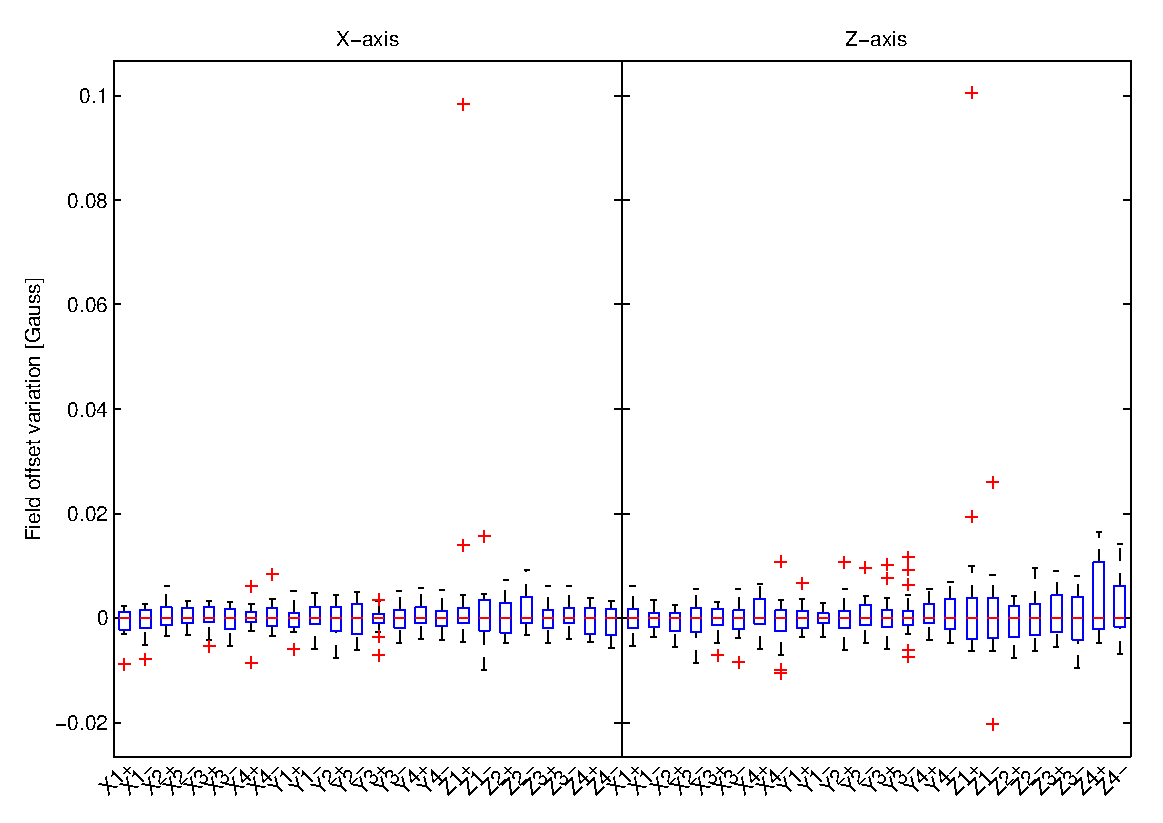
\includegraphics[width=\linewidth]{torqueOffsets}
    \caption{Box Plot from torquer offset test}
    \label{fig:tqoff}
\end{figure}
\end{landscape}}

\Cref{fig:tqoff} shows that there is some variation in the torquer offsets. 

\section{Magnetometer Verification}

There are several steps verify and calibrate the magnetometers on the \acp{SPB}. First the board is tested separate from the rest of the CubeSat. Next the \ac{SPB} is attached to the CubeSat and the torquer compensation routine is run to calculate the torquer offsets. Finally the compensation values are transfered to the \ac{ACDS} board and the compensation is verified.


\subsection{Initial Verification}

The magnetometer verification is done using the Helmholtz cage. The verification is used to test a \ac{SPB} to see if the magnetometer is performing as it should. The \lstinline[style=code,language=Matlab]$spbMag$ function is used for verification. A calibration (see \cref{sec:magcal}) is run on a board separate from the CubeSat. The calibration coefficients are used to calculated parameters found on the datasheed to verify that the magnetometer is performing within specifications. Problems are often caused by bad solder joints which can cause one or more axis to be unresponsive. 

\begin{lstlisting}[caption={\ac{SPB} verification results},label={lst:vspb-res},language=verbatim]
TODO: run command and collect ouput
\end{lstlisting}

\Cref{lst:vspb-res} shows the output from the \ac{SPB} verification. The calculated datasheet parameters are shown along with pass or fail depending on if the values are within the maximums specified by the datasheet.


\subsection{Torquer Compensation}

\label{sec:tq-comp}

The \lstinline[style=code,language=Matlab]$calall$ function is used to calculate the torquer compensation data for a \ac{SPB} and the full set of torquers. The \lstinline[style=code,language=Matlab]$callall$ function calls the \lstinline[style=code,language=Matlab]$tCal$ function three times, once for the X, Y and Z axis. The \lstinline[style=code,language=Matlab]$tCal$ function works similarly to the magnetometer calibration, but the field is swept through the sequence 16 times, once for each torquer state. The data from each sweep is used to calculate the scaling factors for the compensation, $C_1$ $C_2$ $C_4$ and $C_5$ from \cref{eq:magcal}, for all torquer states as well as offset values, $C_3$ and $C_6$ from \cref{eq:magcal}, for each torquer state.

Once calibration values have been calculated for each set of torquers, the values must be combined into a single compensation data set. The scaling factors should be close to the same for the three data sets the scaling factors from each axis are averaged together. The offsets, as described in \cref{sec:tq-comp}, consist of a set of offsets for each set of torquers as well as a common offset. There is one torquer state, ``\texttt{++-{}- ++-{}- ++-{}-}'', that is common to the calibrations in each axis. The static offset is calculated by averaging the values from each axis for the ``\texttt{++-{}- ++-{}- ++-{}-}'' state. The static offset is then subtracted from the offsets for each axis. The scaling factors, common offsets and axis offsets are combined together into a single data set for the magnetometer on each \ac{SPB} which is the compensation data set.

\subsection{Compensation Testing}
\label{sec:tq-comp-tst}

The torquer compensation is tested using the \lstinline[style=code,language=Matlab]$tCalTstFull$ function. The function runs the Helmholtz Cage through a field sequence and takes a magnetometer measurement at each point in the field sequence. During the process a random torquer is flipped every 10 field sequence points. The measurements are corrected, in \matlab, using the compensation data set and compared to the expected field. A plot of the Y+ test data is shown in \cref{fig:tqtst}. The RMS error is also calculated for the data set so the effectiveness of the torquer compensation can be compared to the calibration without torquers.

\begin{figure}[!ht]
    \centering
    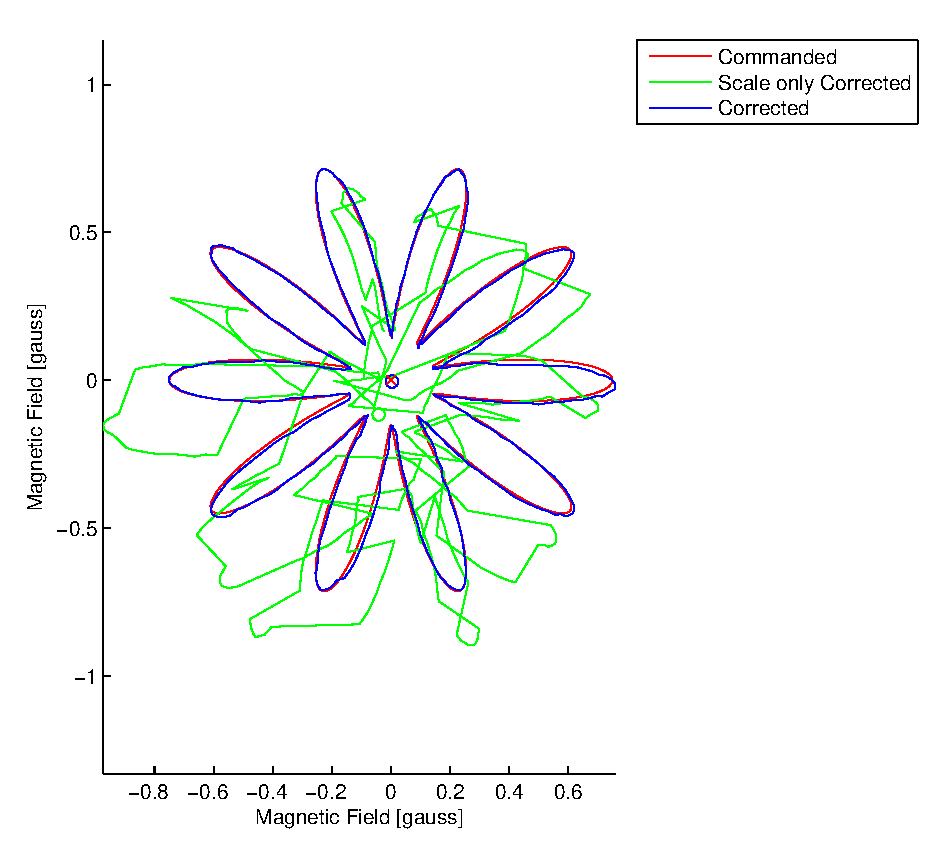
\includegraphics[width=\linewidth]{torqueCalTst}
    \caption{Y+ torquer compensation test showing that the correction provides a large amount of improvement over the uncorrected values}
    \label{fig:tqtst}
\end{figure}

\Cref{fig:tqtst} shows a plot of the Y+ compensation test data. The commanded are the magnetic field values that were programed into the Helmholtz cage. The scale only corrected values are the measurements from the magnetometer corrected using the scaling values from the correction but not the offset values. The corrected values are the measurements from the magnetometer corrected using the full correction data set. The scale only corrected values show that the torquers have corrupted the magnetometer measurements so that, with out the correction values, they can't be used to measure the Earth's magnetic field. The corrected values, however, follow the commanded values much more closely and, while there is a small amount of error visible, appear to be usable for measuring the Earth's magnetic field.

\afterpage{\begin{landscape}
\begin{figure}[p]
    \centering
    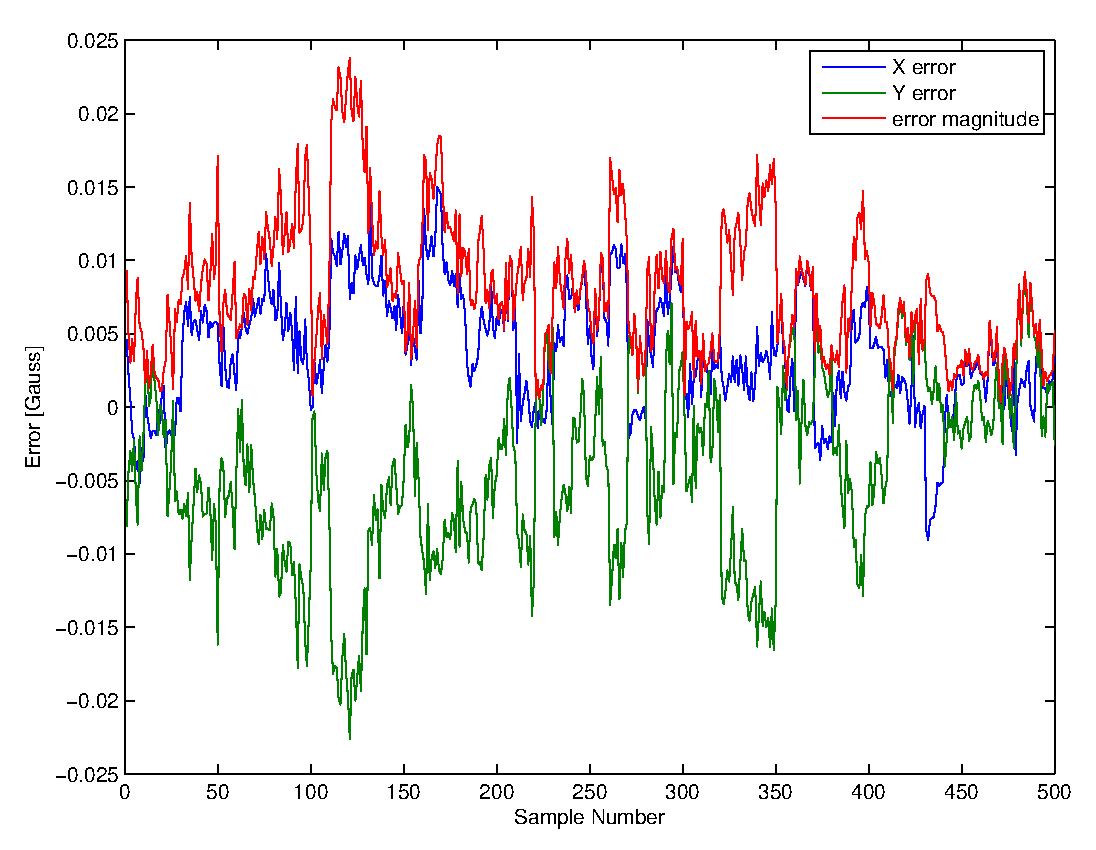
\includegraphics[height=\textwidth]{torqueCalTst-err}
    \caption{Graph showing Y+ torquer compensation error plot}
    \label{fig:tqerr}
\end{figure}
\end{landscape}}

\Cref{fig:tqerr} shows the error for the torquer compensation test. The RMS error for the compensated data is 20~mGauss. The maximum error is 38~mGauss. The RMS error is less than the 26~mGauss to get {\textpm5\textdegree} error but the maximum error of 38~mGauss is much higher. This is likely due to, in part, to the Y+ \ac{SPB} being in a location that gives the highest swing of any other board as shown in \cref{tab:off-stat}.

%\Cref{fig:tqerr} shows the error for the torquer compensation test. The RMS error for the compensated data is 9 mGauss. The maximum error is 24 mGauss. On a 300 mGauss field a 24 mGauss error will cause an angular error of \textpm5\textdegree. The addition of the torquers causes an increase in the RMS and maximum error.
%This can be seen by comparing \cref{fig:tqerr} with \cref{fig:magerr}. In \cref{fig:tqerr} steps in the error are seen as torquers are flipped whereas in \cref{fig:magerr} the error is more consistent across the entire run.

\subsection{Compensation Data Transfer}

The compensation data set is generated in \matlab but to be used in flight it must be stored on the \ac{ACDS} board. The calibration data is stored in the flash memory on the \ac{ACDS} microcontroller. The on-board flash has the benefit of reading the same as \ac{RAM} and is also more abundant but is a bit disruptive to write. This works well in the case of the compensation data because the values are expected to be written once but read often. The other option would be to store the data on the \ac{SD} that is used to log data. In this case the calibration data would need to be buffered in \ac{RAM} which is much more limited than the flash. 

The main flash memory is divided into sectors that are 512 bytes long. Erasing is done on a full sector so the corection data for each \ac{SPB} is stored in its own sector. The correction data is 408 bytes long the header and \ac{CRC} that are stored with the correction data take up 4 bytes leaving 100 bytes wasted. This is not a big deal as there is an abundance of flash memory.

Before the correction data is sent to the \ac{ACDS} it must be repackaged. This is done using the \lstinline[style=code,language=Matlab]$make_cor_dat$ function. Correction data is transfered as single precision IEEE~754 floating point numbers. Because both the \ac{ACDS} processor and most of the machines commonly used to run \matlab are little endian machines, the byte order for the transfered data is little endian. It is important to note that in both ends of the transfer no effort is made to make sure that the data order is correct so this needs to be taken into account if the endianness of one of the machines changes.

The data generated with \lstinline[style=code,language=Matlab]$make_cor_dat$ is temporally stored in the \ac{SD} on the \ac{ACDS} board. The data is stored with an identifier that includes which \ac{SPB} the data is for. On the \ac{ACDS} board the data is unpacked from the \ac{SD}, reformatted slightly, and stored in the on-board flash. 

To simplify the process of generating a calibration set the \lstinline[style=code,language=Matlab]$store_all_cal$ function was written. The \lstinline[style=code,language=Matlab]$store_all_cal$ function generates correction data for all \ac{SPB} boards, sends the data to the \ac{ACDS} and tells the \ac{ACDS} to store the data in flash. 

\subsection{Embedded Compensation Testing}

The test in \cref{fig:tqtst,fig:tqerr} only used the \ac{ACDS} embedded system to flip torquers and take measurements. \matlab was used to do all of the calculations for the calibration. During the flight the calibration must be done with the embedded system on the \ac{ACDS} board. Furthermore the previous tests were for a single \ac{SPB} and could only measure two axes. In flight the measurements from all \acp{SPB} will be combined to get a 3-axis measurement of the magnetic field.

To test the embedded calibration the \lstinline[style=code,language=Matlab]$tCalTstMSP_all$ function is used. To run the test the engineering development prototype of the \ac{ARC}, with compensation data stored on the \ac{ACDS} processor, is placed in the Helmholtz cage. The \lstinline[style=code,language=Matlab]$tCalTstMSP_all$ function operates in much the same way that the \lstinline[style=code,language=Matlab]$tCalTstFull$, explained in \cref{sec:tq-comp-tst}, does. The magnetic field is swept through a field sequence. At every point in the sequence the magnetic field is measured and after every 10 points a random torquer is flipped in each axis. The calibrated total magnetic field values as well as the calibrated values from each \ac{SPB} are read by \matlab and the results are plotted as shown in \cref{fig:tcalMSP,fig:tcalMSPerr,fig:tcalMSPerr-axis}.

\begin{figure}[!ht]
    \centering
    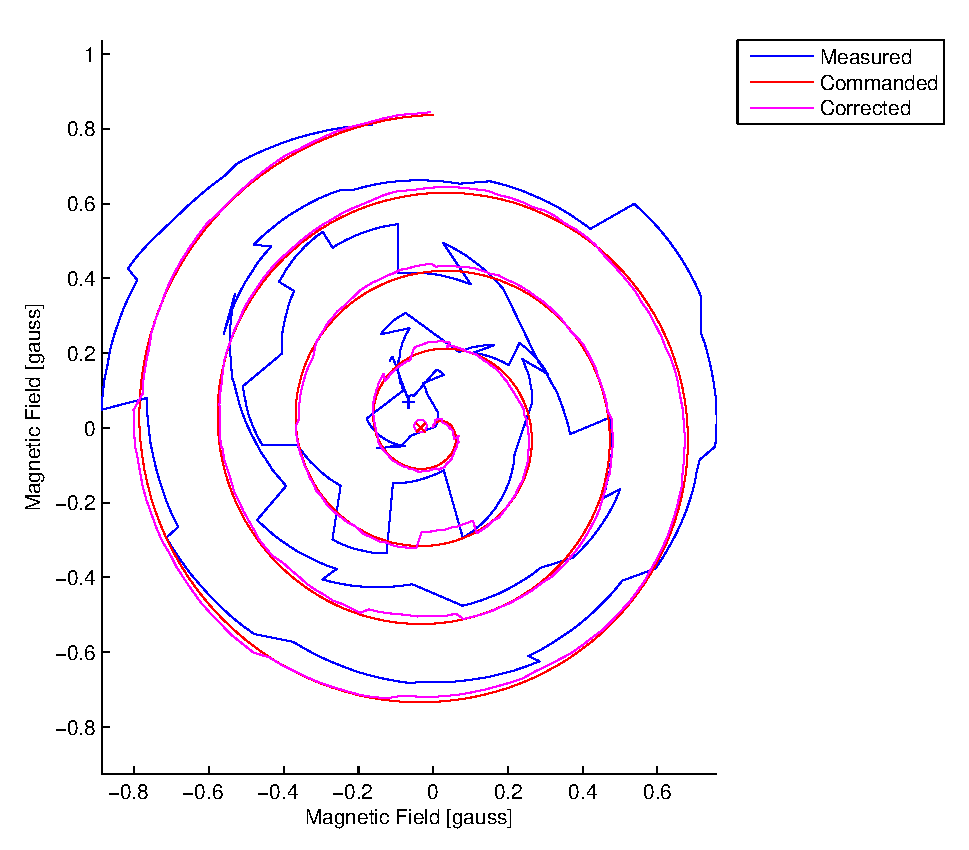
\includegraphics[width=\linewidth]{torqueCalTstMSP}
    \caption{Test of the calibration as performed by the \ac{ACDS} board}
    \label{fig:tcalMSP}
\end{figure}

\Cref{fig:tcalMSP} shows the torquer calibration test using the Y+, Y- and Z+ \acp{SPB} with the calibration performed using the embedded system on the \ac{ACDS} board. The RMS error was 14.6~mGauss. The maximum error was 39.1~mGauss.

\afterpage{\begin{landscape}
\begin{figure}[p]
    \centering
    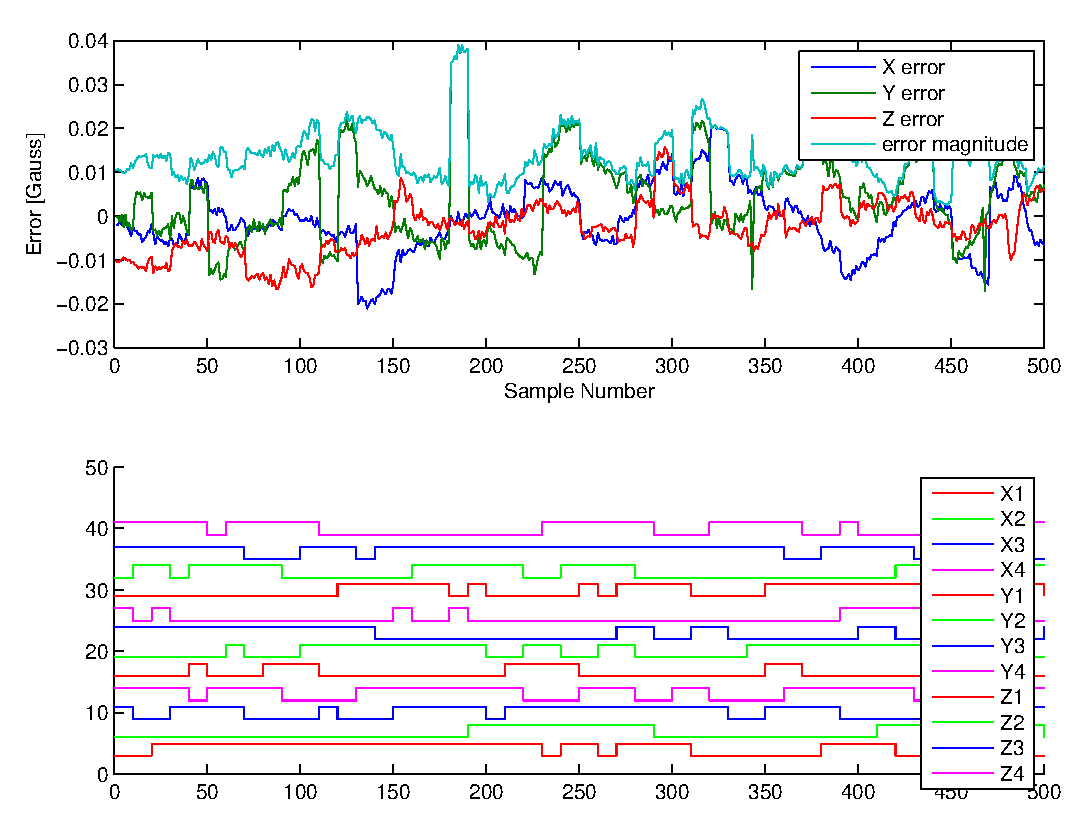
\includegraphics[height=\textwidth]{torqueCalTstMSP-err-flips}
    \caption{Error plot for \cref{fig:tcalMSP} showing torquer states}
    \label{fig:tcalMSPerr}
\end{figure}
\end{landscape}}

\Cref{fig:tcalMSPerr} shows the errors for each sample as well as the torquer states during the samples. The large jumps in the errors all correspond with torquer flips.

\begin{table}[!ht]
    \centering
    \caption{Errors for \ac{ACDS} system calibration test}
    \label{tab:tcalMSPerr}
    \begin{tabular}{|c|c|c|c|}
        \hline
        &X-axis&Y-axis&Z-axis\\
        \hline
        Y+&0.018473&N/A&0.011453\\
        \hline
        Y-&0.007671&N/A&0.009875\\
        \hline
        Z+&0.013049&0.010704&N/A\\
        \hline
        Total&0.007594&0.010704&0.006483\\
        \hline
    \end{tabular}
\end{table}

\Cref{tab:tcalMSPerr} shows the RMS errors in table form. The N/As in the table are because each \ac{SPB} only measures in two axes. For each axis the total error is less than the lowest error from a single axis. This indicates that having multiple measurements of the magnetic field reduces the overall error.

\afterpage{\begin{landscape}
\begin{figure}[p]
    \centering
    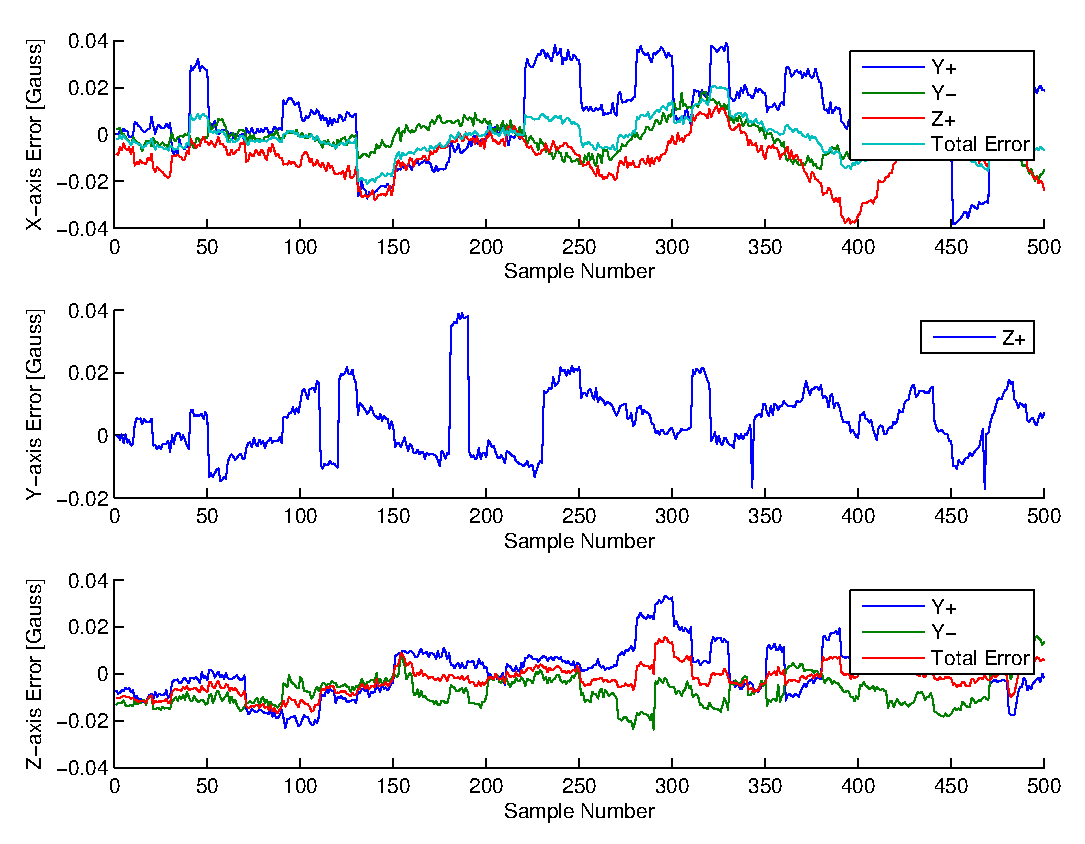
\includegraphics[height=\textwidth]{torqueCalTstMSP-err-axes}
    \caption{Plot of magnetic field errors for each axis}
    \label{fig:tcalMSPerr-axis}
\end{figure}
\end{landscape}}

\Cref{fig:tcalMSPerr-axis} shows the errors from each board in each axis.

\section{B-dot controller simulations}

To verify the B-dot algorithm the \ac{ACDS} is placed in the Helmholtz cage and a rotating field is generated. The minimum rotation rate of the magnetic field that will cause a rotation rate is calculated by starting with \cref{eq:bdot-cross}

\begin{equation}
    \dot{\vec{B}} = \vec{B} \cross \omega
    \label{eq:bdot-cross}
\end{equation}

If the axis of rotation is perpendicular to the field rotation then \cref{eq:bdot-cross} becomes \cref{eq:bdot-mul}

\begin{equation}
    \dot{\vec{B}} = \left| \vec{B} \right| \cdot \left| \omega \right|
    \label{eq:bdot-mul}
\end{equation}

The B-dot algorithm equation is shown in \cref{eq:bdot-alg}.

\begin{equation}
    M_{cmd} = C \dot{\vec{B}} 
    \label{eq:bdot-alg}
\end{equation}

Substituting \cref{eq:bdot-mul} into \cref{eq:bdot-alg} and solving for $\omega$ gives \cref{eq:omega-th}. Where $M_{th}$ is the torque switching threshold for the torquers and $\omega_{th}$ is the minimum rotation rate required to flip a torquer.

\afterpage{\begin{landscape}
\begin{figure}[p]
    \centering
    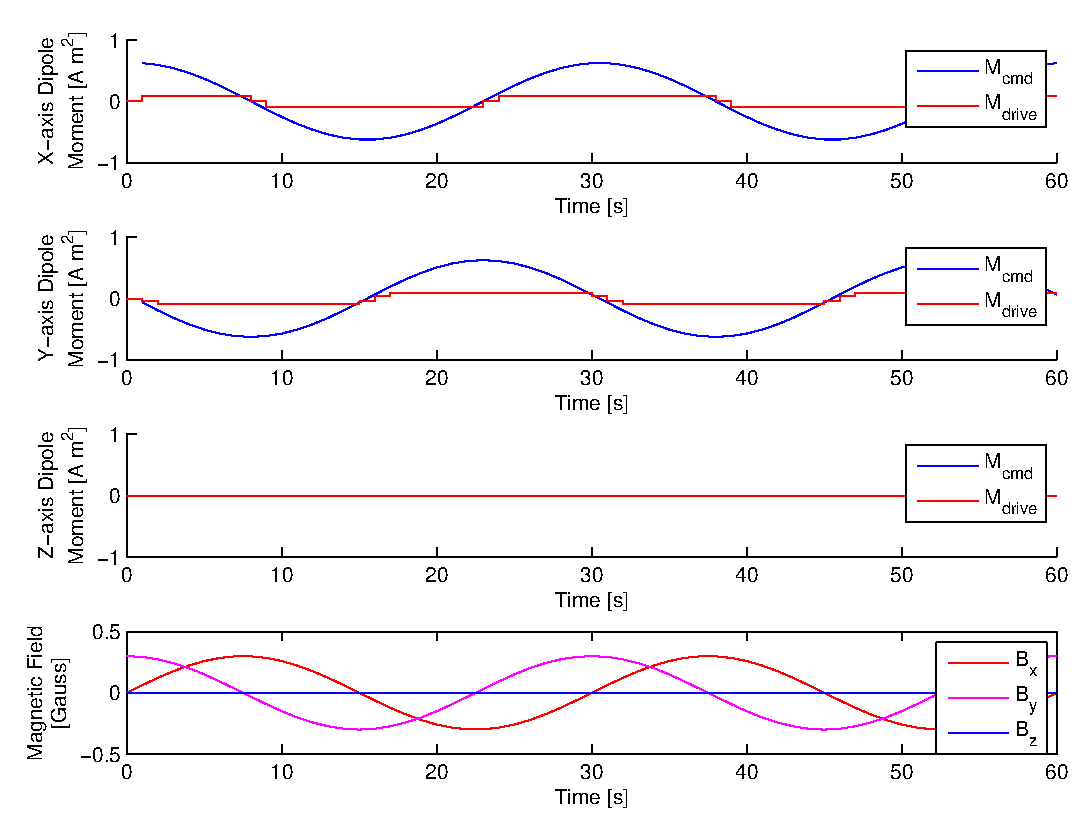
\includegraphics[height=\textwidth]{detumble-sim}
  \caption{Simulation of torquer output with spinning magnetic field}
    \label{fig:detumble-sim}
\end{figure}
\end{landscape}}

\begin{equation}
    \omega _ {th} = {M _ {th} \over{ {C \left| \vec{B} \right|}}}
    \label{eq:omega-th}
\end{equation}

If a 0.3 gauss field is used and $C$ is 4 and the torquer switching threshold is $0.022 \unit{A \cdot m} ^2$ then $\omega_{th}$ is calculated as follows

\begin{equation}
    \omega _ {th} = { 0.022 \over{ {4 \cdot 0.3}}} = 0.0183 ~ \unit{rad / sec}
\end{equation}

To understand what the response of the \ac{ACDS} to a rotating magnetic field should be, a simulation was written. The simulation simply generates a magnetic field sequence and uses the B-dot algorithm to determine what the magnetic torque should be. The simulation quantizes the output torque but does not enforce the one flip per time step requirement.

%With the field set to $\omega_{th}$ a torquer should flip as $\dot{\vec{B}}$ becomes aligned with a torquer axis as the field continues to sweep the torquer will switch off.

\Cref{fig:detumble-sim} shows a simulation of the detumble algorithm in a spinning magnetic field. The field has a magnitude of 0.3~Gauss spins around the Z-axis. The gain of the simulated controller was -4. The plots show the magnetic dipole moment that the algorithm wants to drive and is able to drive as the magnetic field spins around.


\section{Detumble Flip Test}

To test the detumble algorithm on the \ac{ACDS} hardware the \lstinline[style=code,language=Matlab]$bdot_test$ function is used. A timer is used to update the magnetic field in the Helmholtz cage every half second. The field is set to a field that by default rotates around the Z-axis at 2~rpm. The \ac{ACDS} is set to operate in detumble mode and the data that the \ac{ACDS} outputs is captured.

\afterpage{\begin{landscape}
\begin{figure}[p]
    \centering
    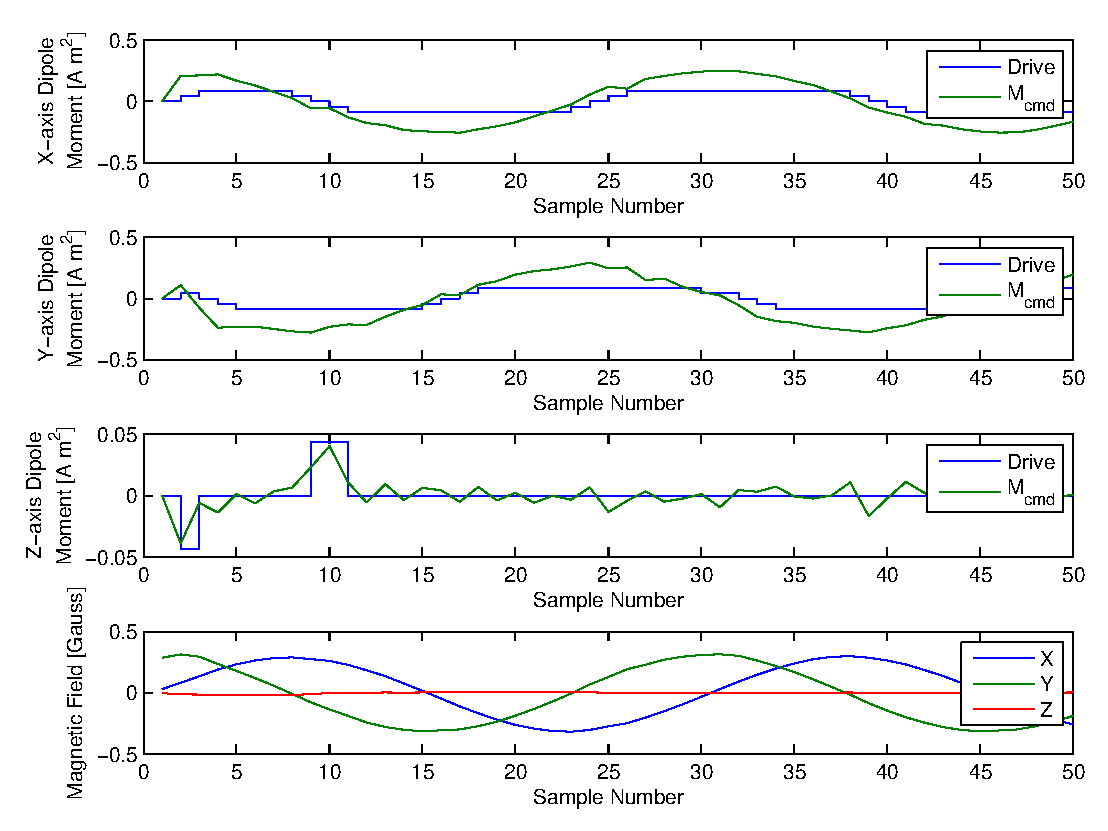
\includegraphics[height=\textheight]{detumble-test}
  \caption{Test of the B-dot controller}
    \label{fig:detumble-test}
\end{figure}
\end{landscape}}

\Cref{fig:detumble-test} shows the results of the detumble test. This is the same as the detumble simulation in \cref{fig:detumble-sim} except the field has been programed into the Helmholtz cage, measured by the \acp{SPB}, calculations done by the \ac{ACDS} and torquers flipped in an attempt to stop the motion.

The results in \cref{fig:detumble-test} are similar to the results in the simulation in \cref{fig:detumble-sim}. The main difference is that there are some unexpected flips in the Z-axis. This is due to noise in the magnetic field causing torquers to be flipped. It is unclear if the noise is caused by the environment in the Helmholtz cage or by torquer flips and imperfect torquer calibration.


